\documentclass[../main.tex]{subfiles}
\begin{document}

\section{Optimal Control of Pitch/Travel with Feedback (LQ)}
In this task we add feedback to the optimal controller that we developed in \cref{kap:Part2OptimalControlWithoutFeedback}.

\subsection{Motivation}
The experimental results in \cref{kap:task_10_2_experimental_results} clearly shows that planning a sequence of inputs does not produce the expected sequence of outputs - as that section explains there are many reasons for travel-drift. In situations with drift without feedback then the output will not follow the planned trajectory, but adding feedback could compensate for the drift and offset and therefore reduce or eliminate the deviation from the planned trajectory.

The results achieved in this section shows that adding feedback greatly improves performance.

\subsection{Introducing feedback}
There are many approaches to adding feedback, but in this assignment only two will be considered: linear state feedback and model predictive control.

\textbf{Linear state feedback} adds a new control layer below the optimization layer, the advanced control layer, that controls the setpoint to the pitch controller. The setpoint is determined from a control law that considers the optimal trajectory and the current state of the system. If the states deviate from the optimal value the input is changed according to the pitch-control equation:
\begin{equation}\label{eq:lab3_feedback}
	u_k = u_k^* - \bm{K}^T(\bm x_k - \bm x_k^*)
\end{equation}
where $u_k^*$ and $\bm x_k^*$ are the optimal input and state trajectories predicted in the optimization layer, $u_k$ is the next input and $x_k$ is the current state. $K$ is the linear state feedback gain. 

In this exercise the gain matrix $K$ is calculated as an infinite horizon LQ controller, see \cref{kap:task_10_3_LQ_controller} for more info about the exact implementation.

\textbf{Model Predictive Control (MPC)} is a completely different solution: the optimal trajectory is recalculated at every timestep - instead of compensating for deviation from optimal, the optimal is recalculated to get a new possible trajectory based on the current states. See \cref{kap:10_3_mpc} for more info about how that could be implemented here.

\subsection{LQ controller} \label{kap:task_10_3_LQ_controller}
A Linear Quadratic (LQ) controller minimizes the quadratic objective function:
\begin{equation}
    J = \sum^\infty_{i=0} \Delta x_{i+1}^\top Q \Delta x_{i+1} + \Delta u_i^\top R \Delta u_i, \quad Q \ge0, \quad R > 0
\end{equation}
for a linear model
\begin{equation}\label{eq:lab3_lin_model}
	\Delta x=A\Delta x_i + B \Delta u_i
\end{equation}
Here $ \Delta x = x - x^*$ and $\Delta u = u - u^*$ are deviations from the optimal trajectory.

This formulation is an infinite horizon linear quadratic regulator which has a solution with a constant linear feedback gain, $K$ - which is exactly what was specified previously! Note that this regulator does not have any constraints.

\subsubsection{Choosing the weights}
The matrix $Q$ and the scalar $R$ are the weights of the optimalization problem. $Q$ determines how much state-deviations should be penalized, while $R$ determines how much input-deviation should be penalized. What needs to prioritized depends on the application.

In this case the system is a helicopter where the goal is to control the travel of the helicopter. The travel is the most important state, while travelrate, pitch and pitchrate are secondary. Thus it makes sense to prioritize keeping travel close to the planned trajectory - it is of course not possible to keep all states close to the trajectory. This motivates a \textbf{state-weight} with relatively high value related to travel.

The LQR regulator controls the pitch-setpoint that in turn controls travel. In the end controlling travel is the most important - a deviation in setpoint from the predicted optimal is completely fine as this is how travel is regulated. Thus a low input-weight is warranted as that allows the setpoint to deviate further from the planned trajectory.

\subsubsection{Respecting constraints}
The pitch-setpoint in the optimalization layer has a constraint, see \cref{sec:lab2_constraints} - but the implementation of LQR controller does not respect this constraint! The result is that the pitch-setpoint could fall outside the constraint imposed in the optimalization layer. This does in fact happen, for instance in \cref{fig:LAB3_Q_variations_travel}, where the setpoint is outside the constraint ($\approx 0.52 rad $).

The simplest solution to this problem is to respect the constraint by saturating the output of the regulator to that value. However that does makes impossble for the LQ regulator to compensate in cases where the input is already constrained, therefore it would make sense to set the saturation limit slightly higher than the constraint value to allow the regulator to work in such cases (or equivalently set the constraint lower than the saturation point).

\subsubsection{Calculating the solution}
Calculating the solution to the LQR problem is trivial using Matlab:
\begin{lstlisting}[language=Matlab]
% The discrete system described as a state space system, Ad and Bd must be defined

% W1 is the weigth of travel
% W2 is the weight of travelrate
% W3 is the weight of pitch
% W4 is the weight of pitchrate
Q = diag([W1, W2, W3, W4]);

% W5 is the weight of the input
R = W5;

% The function dlqr is used to solve the LQR problem
[K, S, e] = dlqr(Ad, Bd, Q, R);
\end{lstlisting}

\subsection{Model Predictive Control}\label{kap:10_3_mpc}
Model Predictive Control is another way of introducing feedback to an optimal control system. In an MPC controlled system the optimal response and input is recalculated at every timestep, the input used is simply the first of the optimal input values calculated at every step.

This is a drastically different approach to the LQ-method impemented in this laboratory exercise.

\subsubsection{Implementing MPC}
Implementing MPC requires a system model, cost function, current state and input control.

One could make a Matlab function that the simulink model uses at every timestep. The input to this function is the current state (either measured or estimated), while the output is connected to the pitch-regulator. The function itself has a model of the system as well as the cost function - with the state from the system the optimalization problem can be solved and the first system-input is returned to the simulink model. 

\subsubsection{Advantages of MPC}
The biggest advantage of MPC compared to the linear state feedback introduced here is that MPC generates a new optimal trajectory that is possible to achieve - this is very imporant.

Imagine a situation where the helicopter needs to fly below some obstacle. A deviation in elevation that would cause a collision with the obstacle might not be corrected before travel reaches the obstacle - MPC would slow down travel enough to have a trajectory that is possible to achieve.

\subsubsection{Disadvantages of MPC}
The biggest disadvantage to MPC is complexity and computation time - in a control system there are hard deadlines and if the optimalization problem has not been solved in that deadline the system has a problem.

First of all the problem must be simple enough or optimized enough to solve at every timestep, else the problem must be simplified, optimized or the timestep must be increased. The time to solve a problem can also vary, which makes this issue more complex.

Another issue is \textbf{existance of solutions} must be guaranteed for all situations. It is possible to have problems that have solutions in some state and reference values, while being undefined for others. This could cause the helicopter to freeze mid-air because there was no solution.

\subsubsection{Modified Control Hierarchy with MPC}

\missingfigure{Modified control hierarchy}

\subsection{Experimental results}\label{sec:lab3_result}
The group performed a host of controlled tests with different tunings within five different targets:
\begin{enumerate}
	\item Prioritizing input use, see \cref{fig:LAB3_R_variations}
	\item Prioritizing travel, see \cref{fig:LAB3_Q_variations_travel}
	\item Prioritizing travelrate, see \cref{fig:LAB3_Q_variations_travelrate}
	\item Prioritizing pitch, see \cref{fig:LAB3_Q_variations_pitch}
	\item Prioritizing pitchrate, see \cref{fig:LAB3_Q_variations_pitchrate}
\end{enumerate}

It is very clear that introducing feedback produced results much better than the ones achieved without feedback, almost regardless of the tuning of the LQR regulator.

Prioritizing input usage only has a slight effect, the input usage does get slightly closer to the planned trajectory but not by much. This could of course be pushed further by weighing states lower or input higher, but this was not explored - if the input is regulated very close to the planned trajectory then the result is the same as the previous lab-exercise where u was exactly equal to the planned trajectory.

Prioritizing travel has a great effect on the travel response - resulting in almost perfect travel response. Unfortunately this also introduced oscillations in pitch-setpoint, pitch and pitchrate.

Prioritizing travelrate, pitch and pitchrate results in responses closer to the corresponding planned trajectory, but this is not further discussed as travel is the state most important to control - theese experiments were only to show that it would be possble should another state be valuable.

\subsubsection{Possible improvements}
The group observed that the state never reached the optimal trajectory, even with very high Q-values. The group believes that adding integration to the LQ-regulator would eliminate the stationary offset between travel and the planned travel trajectory.

Another possible improvement would be to change the cost function in the optimalization layer to generate a trajectory that is easier for the helicopter to follow. There is not guarantee that it is physically possible for the helicopter to follow the trajectory generated here, because the model of the system is not perfect.

\subsubsection{Plots}

\begin{figure}[h]
	\centering
    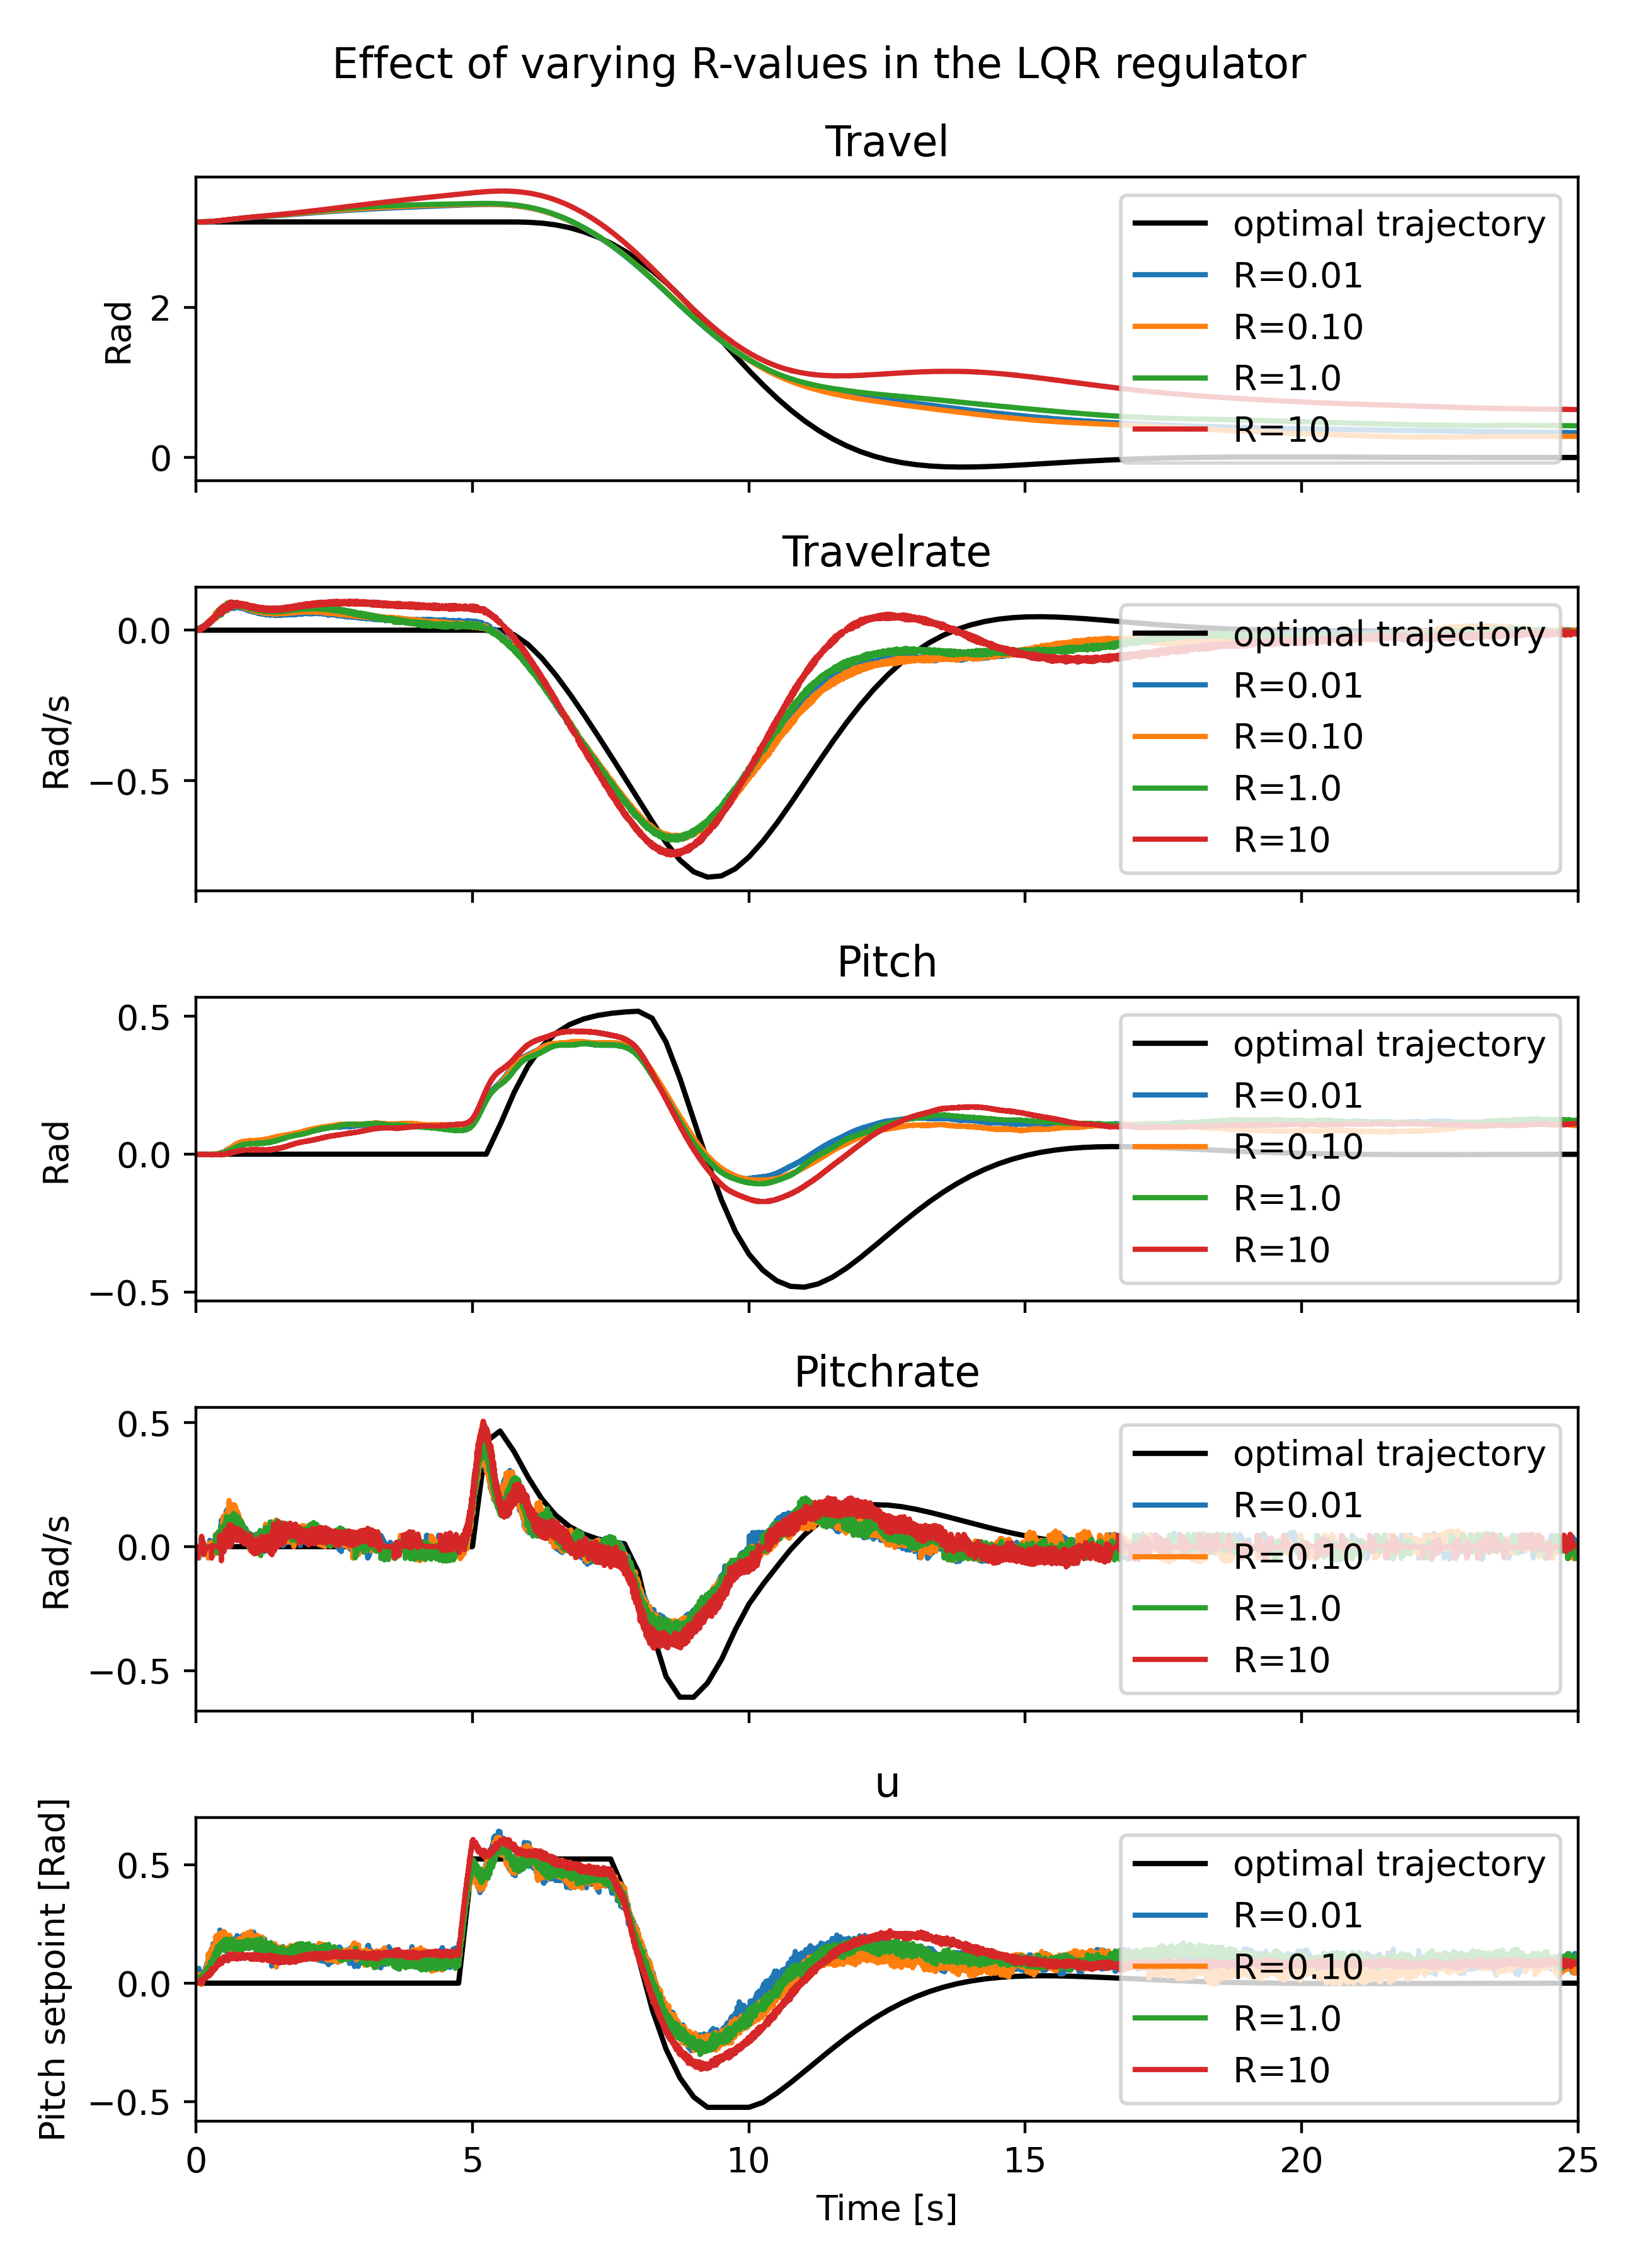
\includegraphics[width=0.8\linewidth]{figures/LAB3_R_variations.png}
	\caption{Prioritizing input-usage while keeping Q=diag([1,1,1,1]). This shows a very slight difference between weights. No further experimentation was done because if $u_k = u_k^*$ then that would be the same as the previous exercise.}
	\label{fig:LAB3_R_variations}
\end{figure}

\begin{figure}[h]
	\centering
	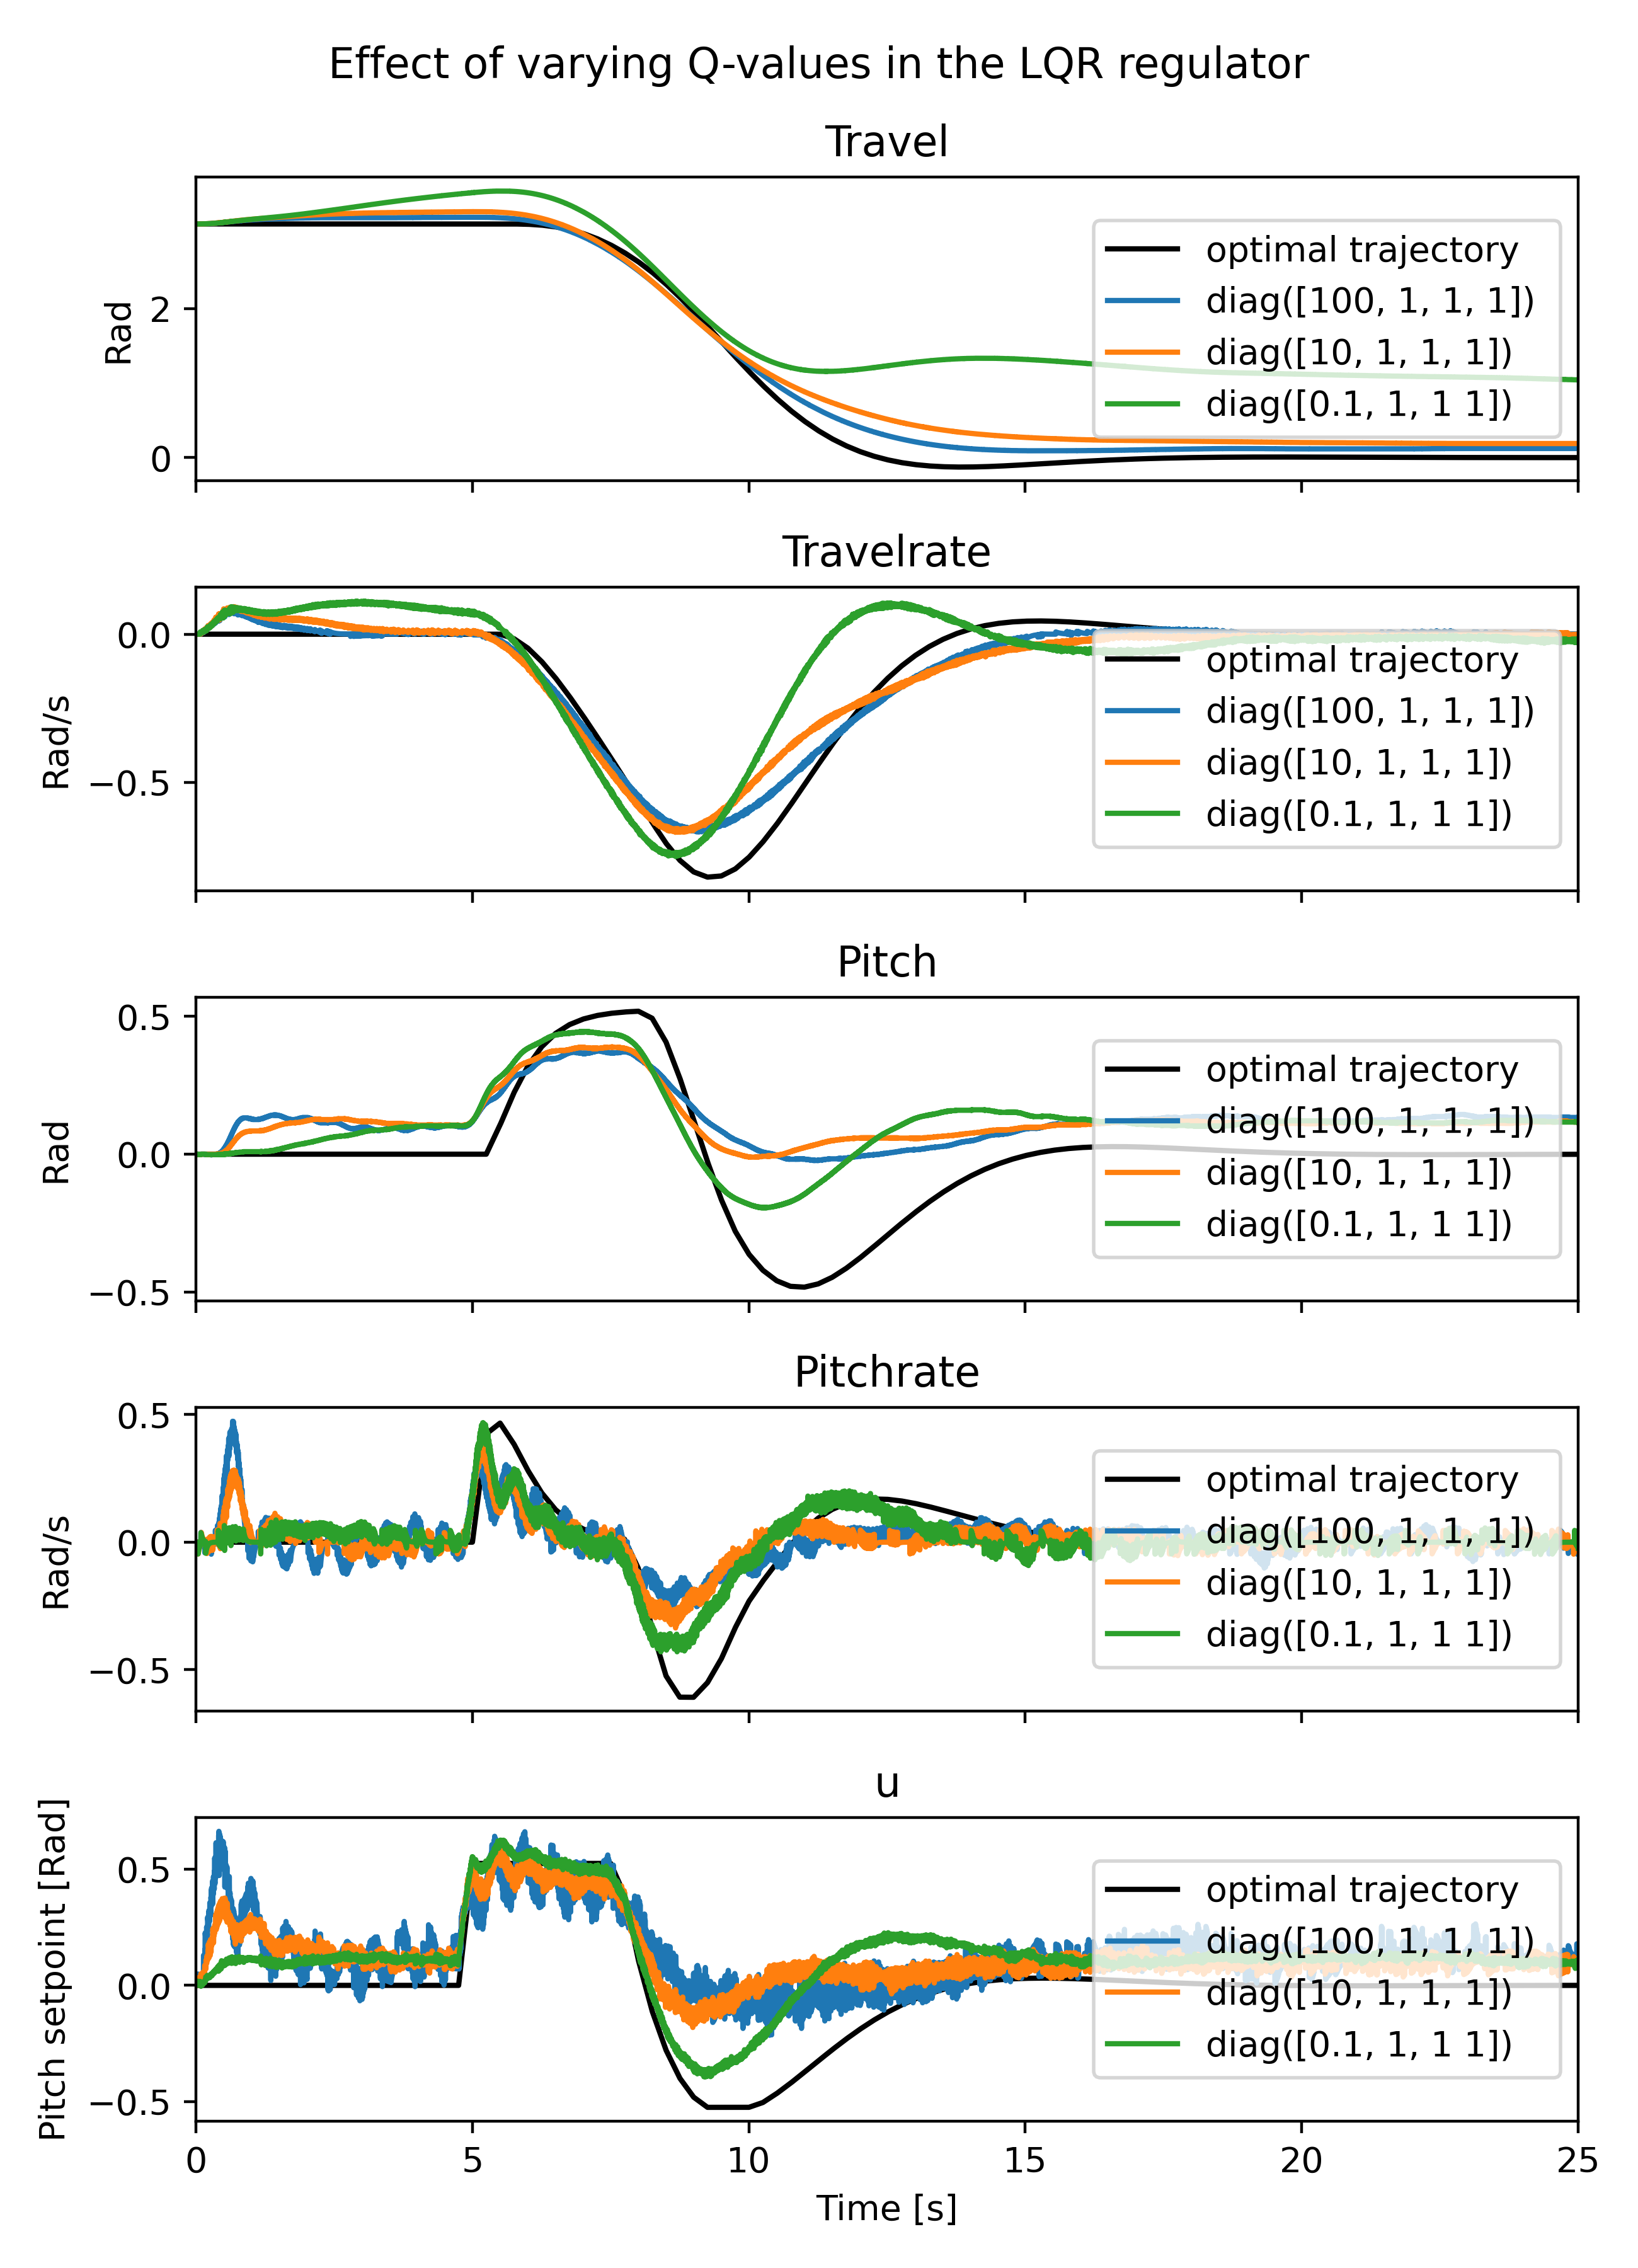
\includegraphics[width=0.8\linewidth]{figures/LAB3_Q_variations.png}
	\caption{Prioritizing the weight related to travel while keeping $R=1$. This was very effective in reducing offset between travel and the planned trajectory. Unfortunately at heigher gains there is some offset introducted and even then there is still a constant offset. A regulator with integral action would probably eliminate this offset without introducting oscillations.}
	\label{fig:LAB3_Q_variations_travel}
\end{figure}

\begin{figure}[h]
	\centering
	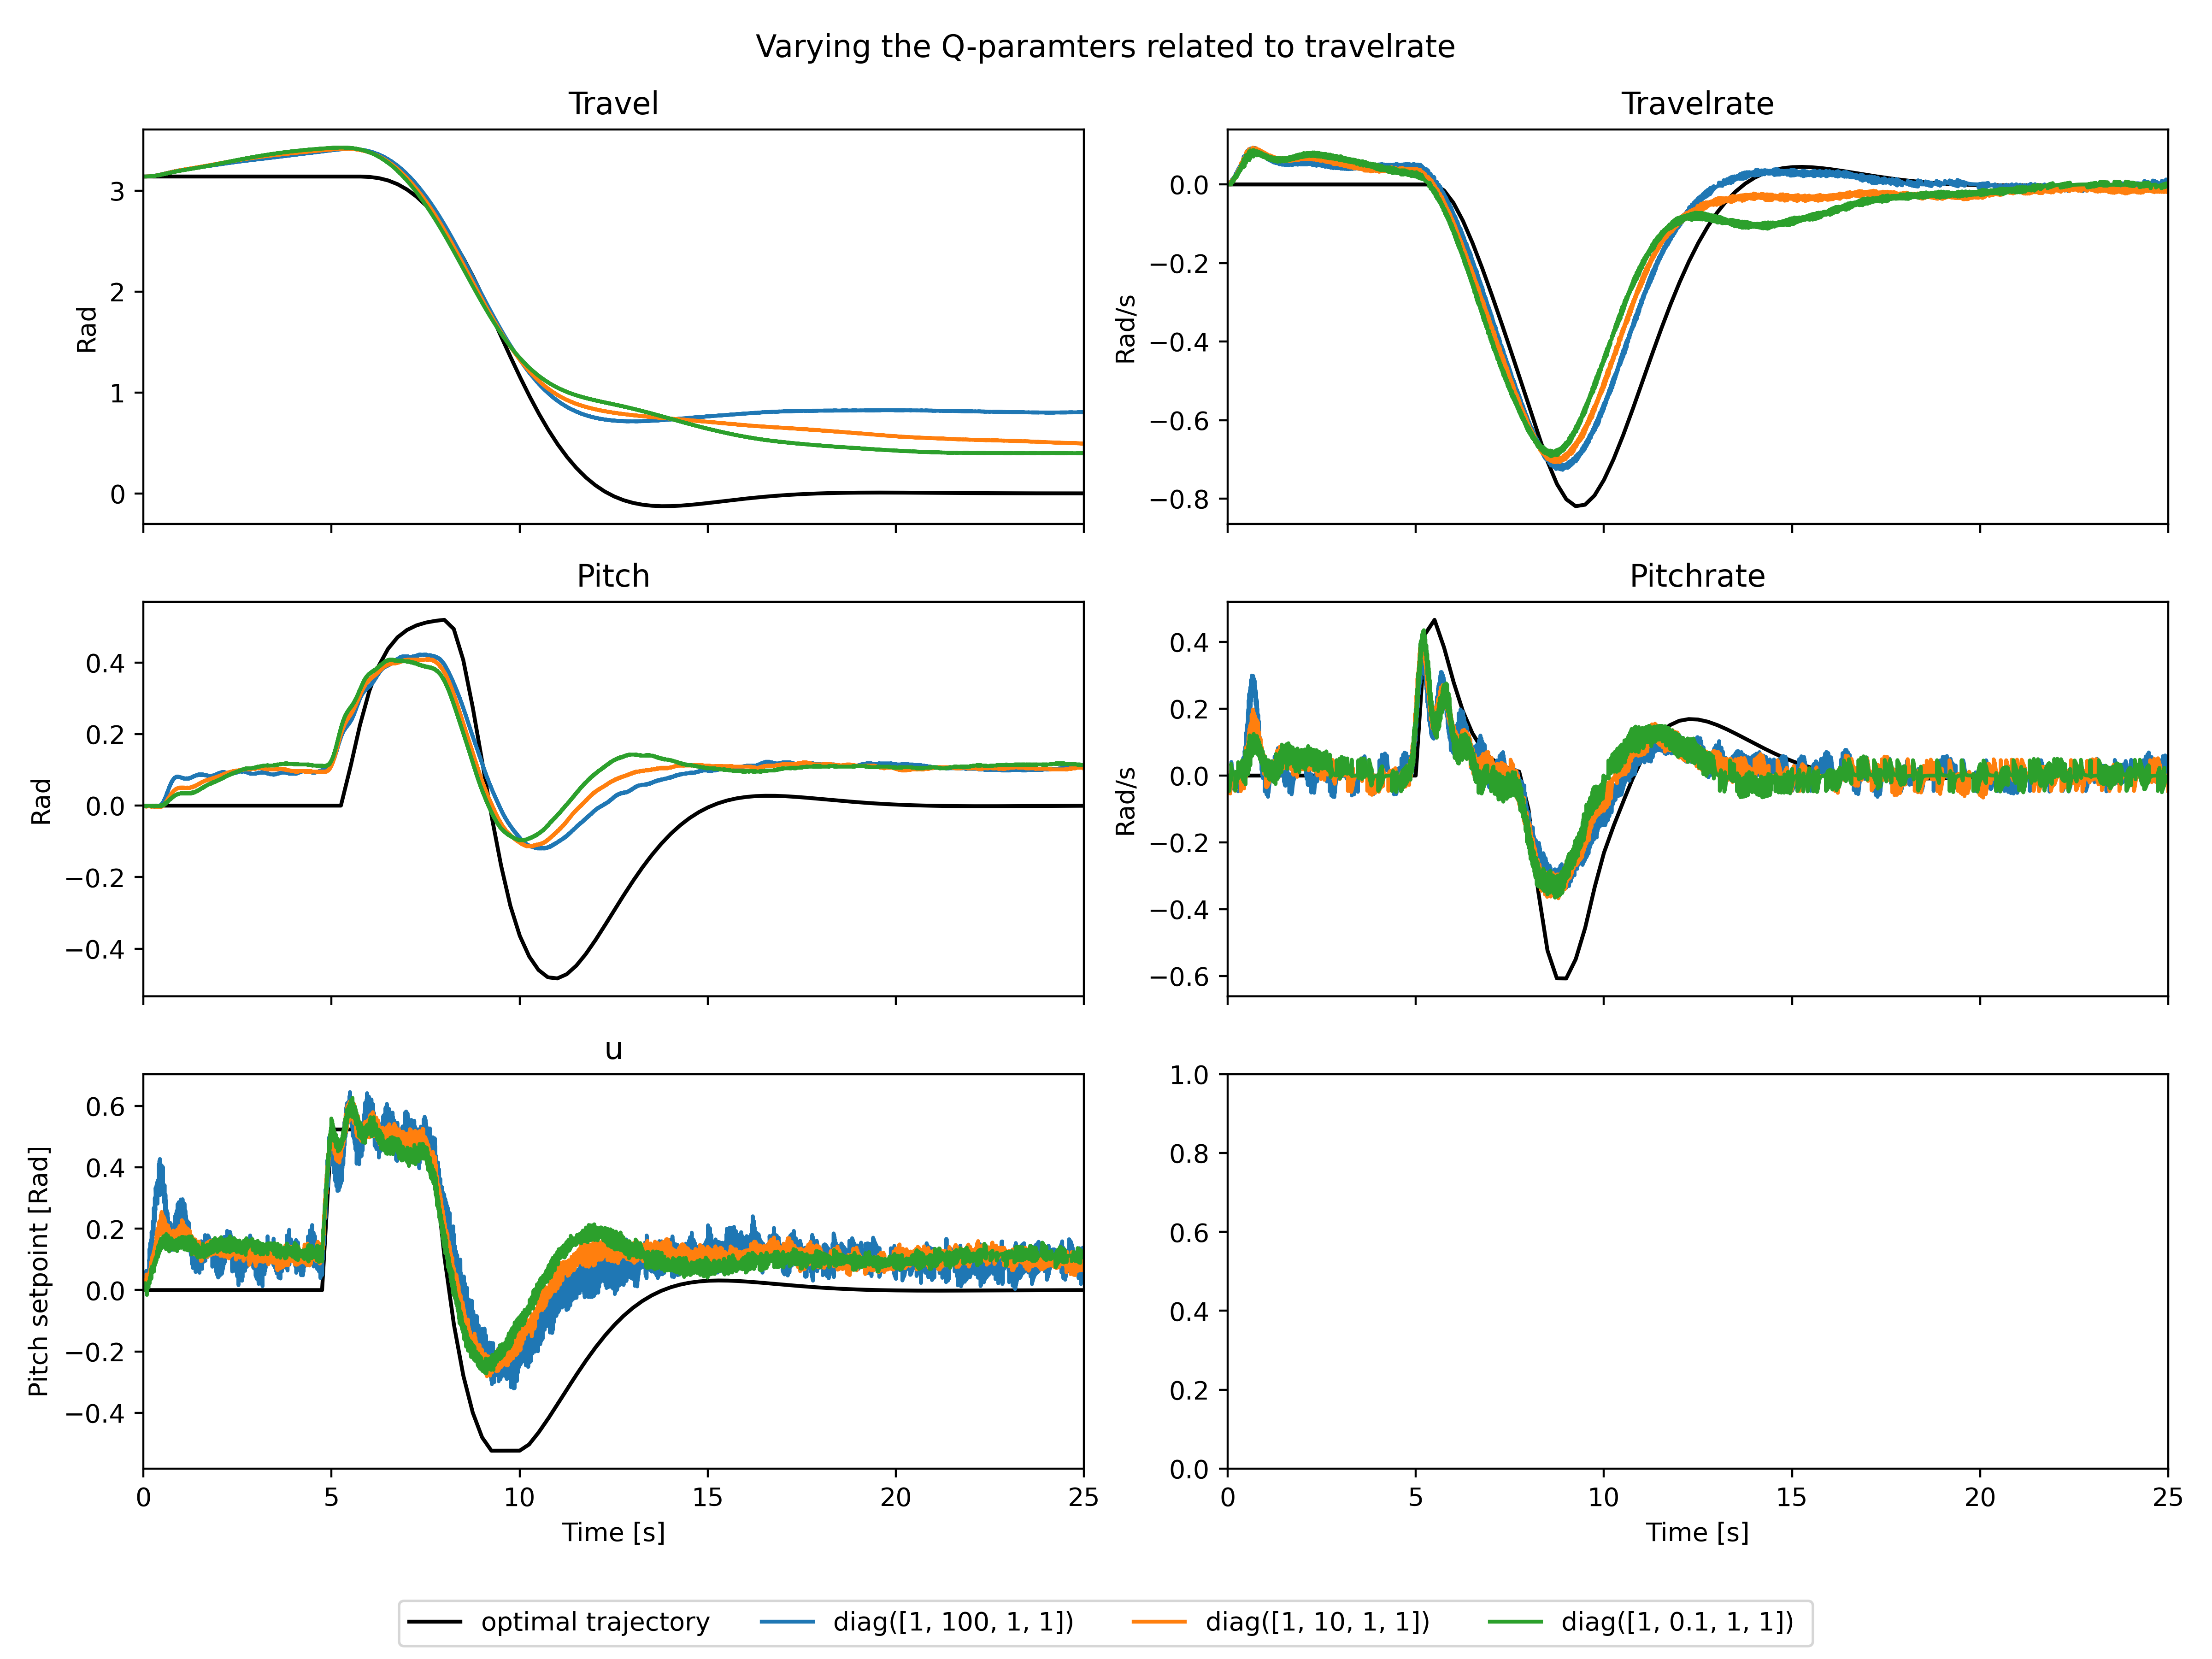
\includegraphics[width=0.8\linewidth]{figures/LAB3_Q_variations_travelrate.png}
	\caption{Changing the weight of the travelrate state, $R=1$. This had only a minor effect with small variations in the response.}
	\label{fig:LAB3_Q_variations_travelrate}
\end{figure}

\begin{figure}[h]
	\centering
	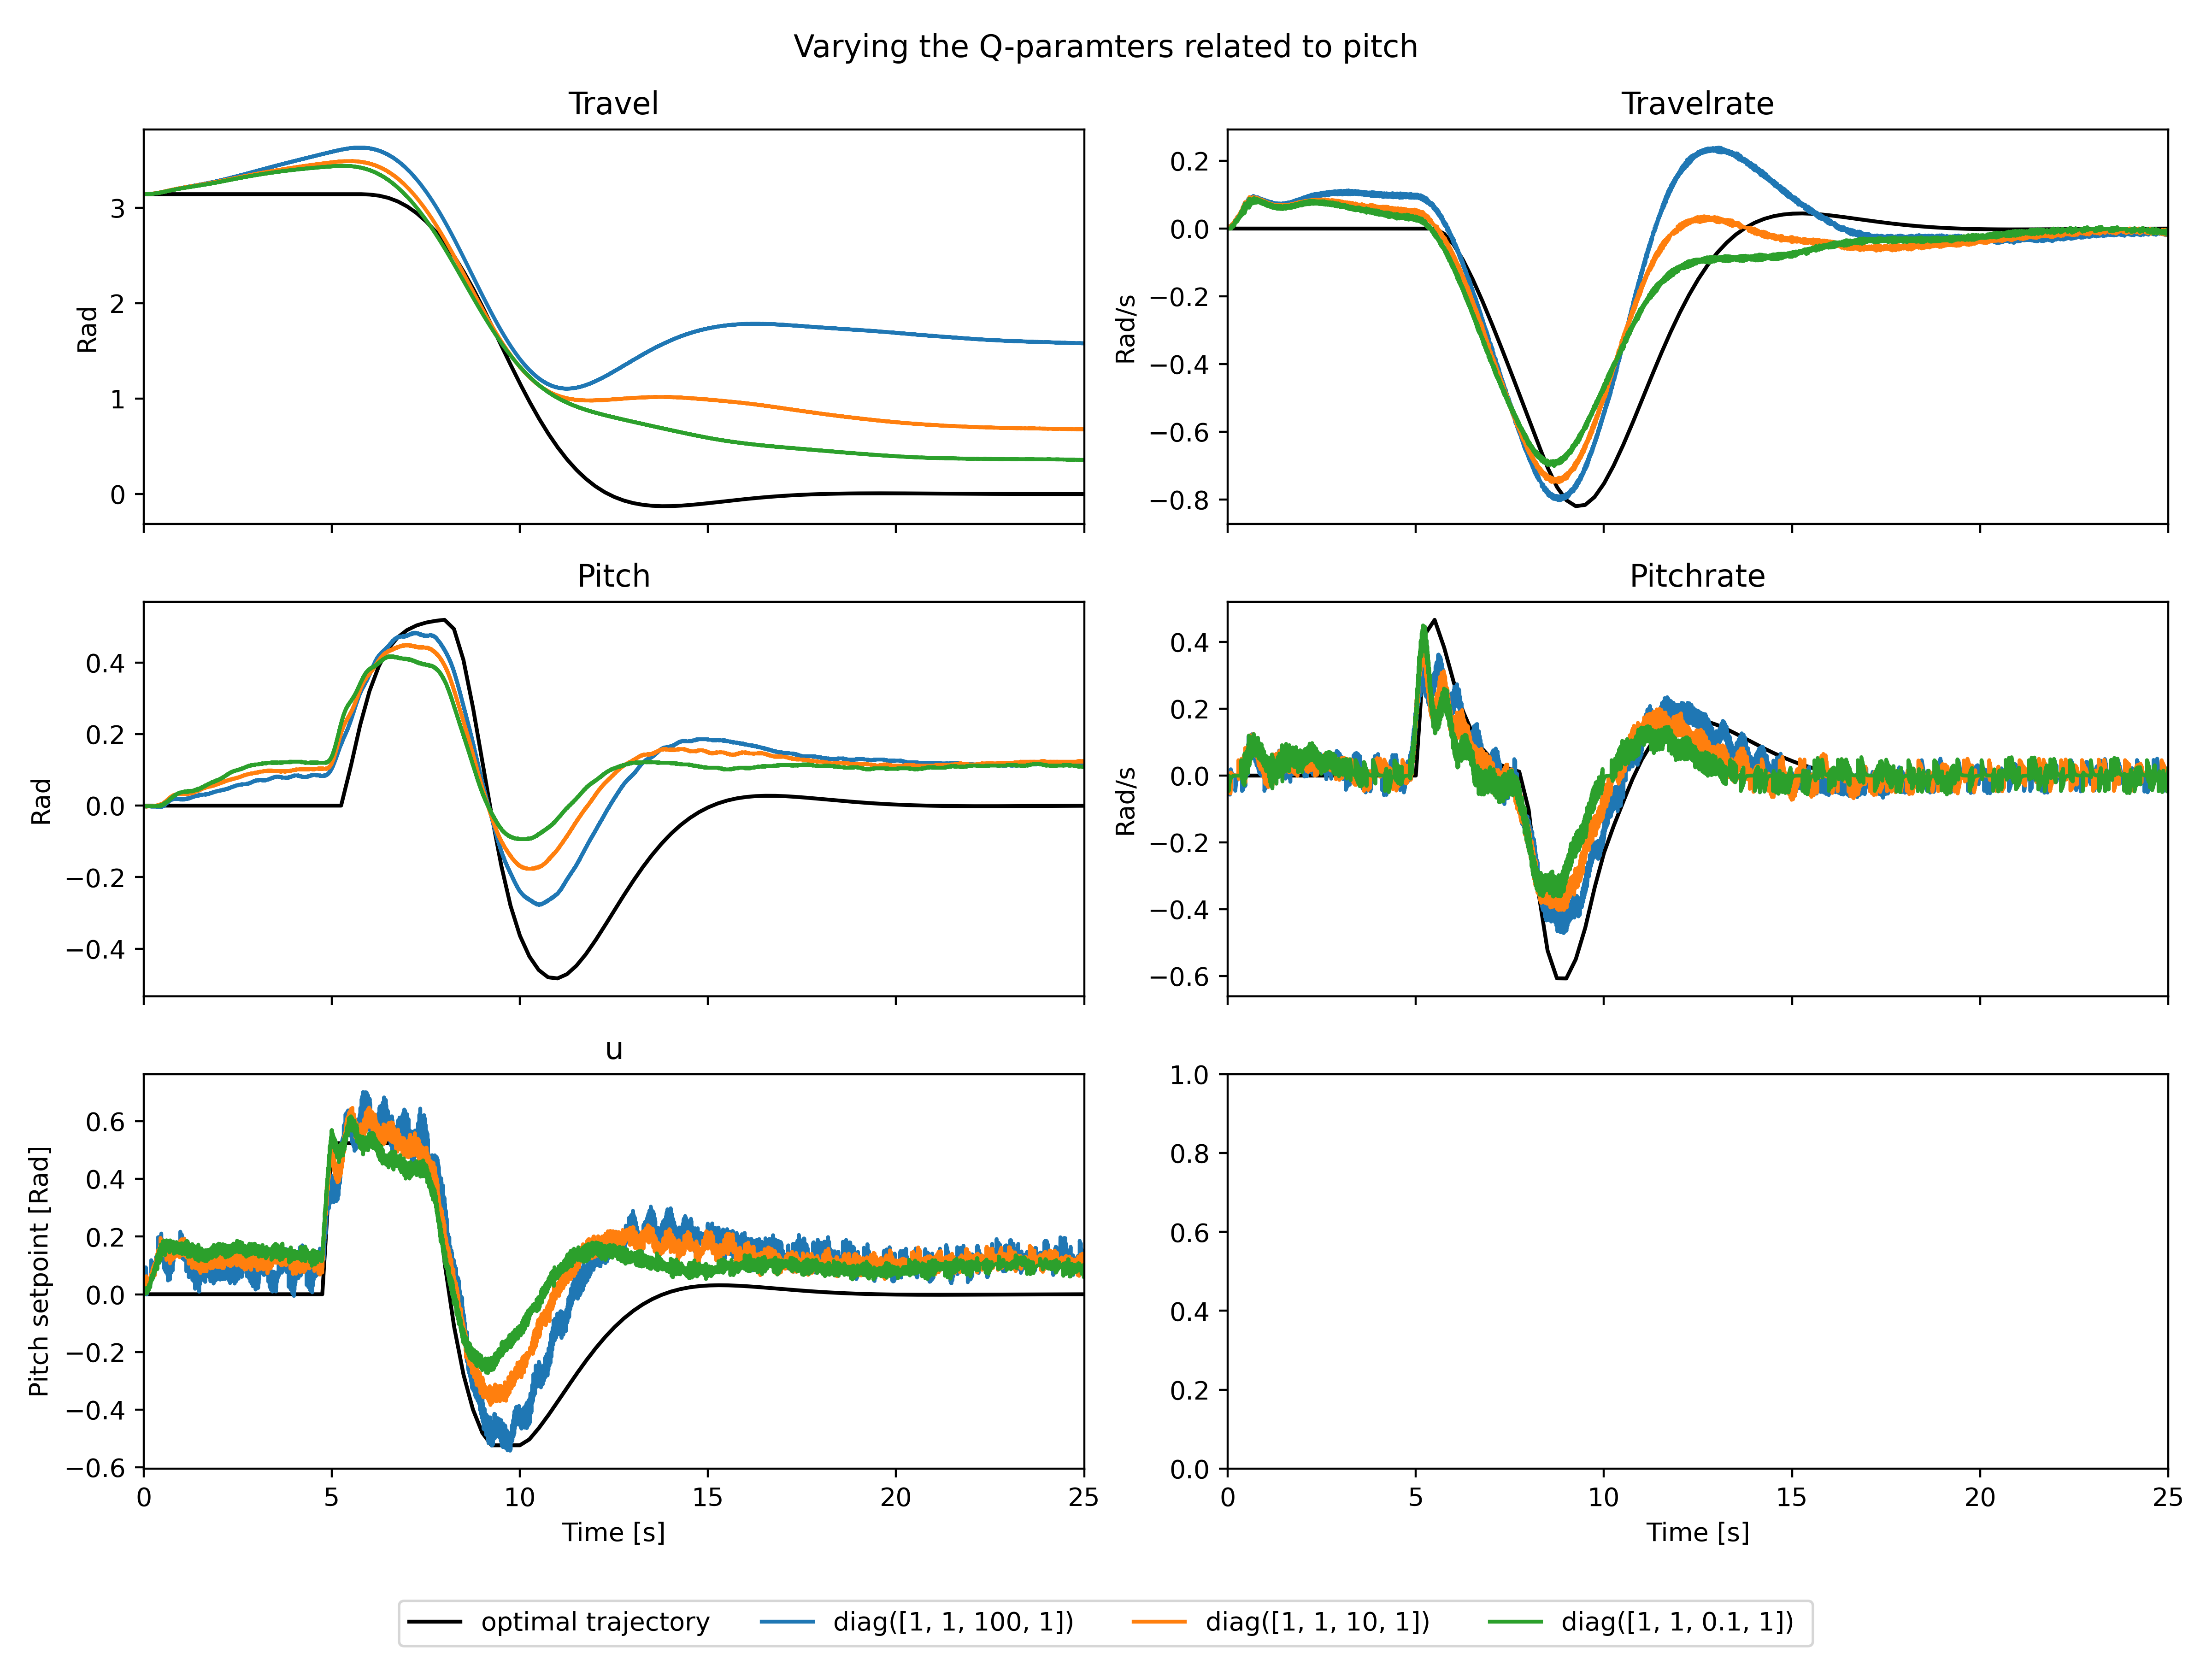
\includegraphics[width=0.8\linewidth]{figures/LAB3_Q_variations_pitch.png}
	\caption{Changing the weight of the pitch state, $R=1$. This had the effect of getting both pitch, pitch-setpoint and pitchrate closer to the planned trajectory at the expense of travel and travelrate.}
	\label{fig:LAB3_Q_variations_pitch}
\end{figure}

\begin{figure}[h]
	\centering
	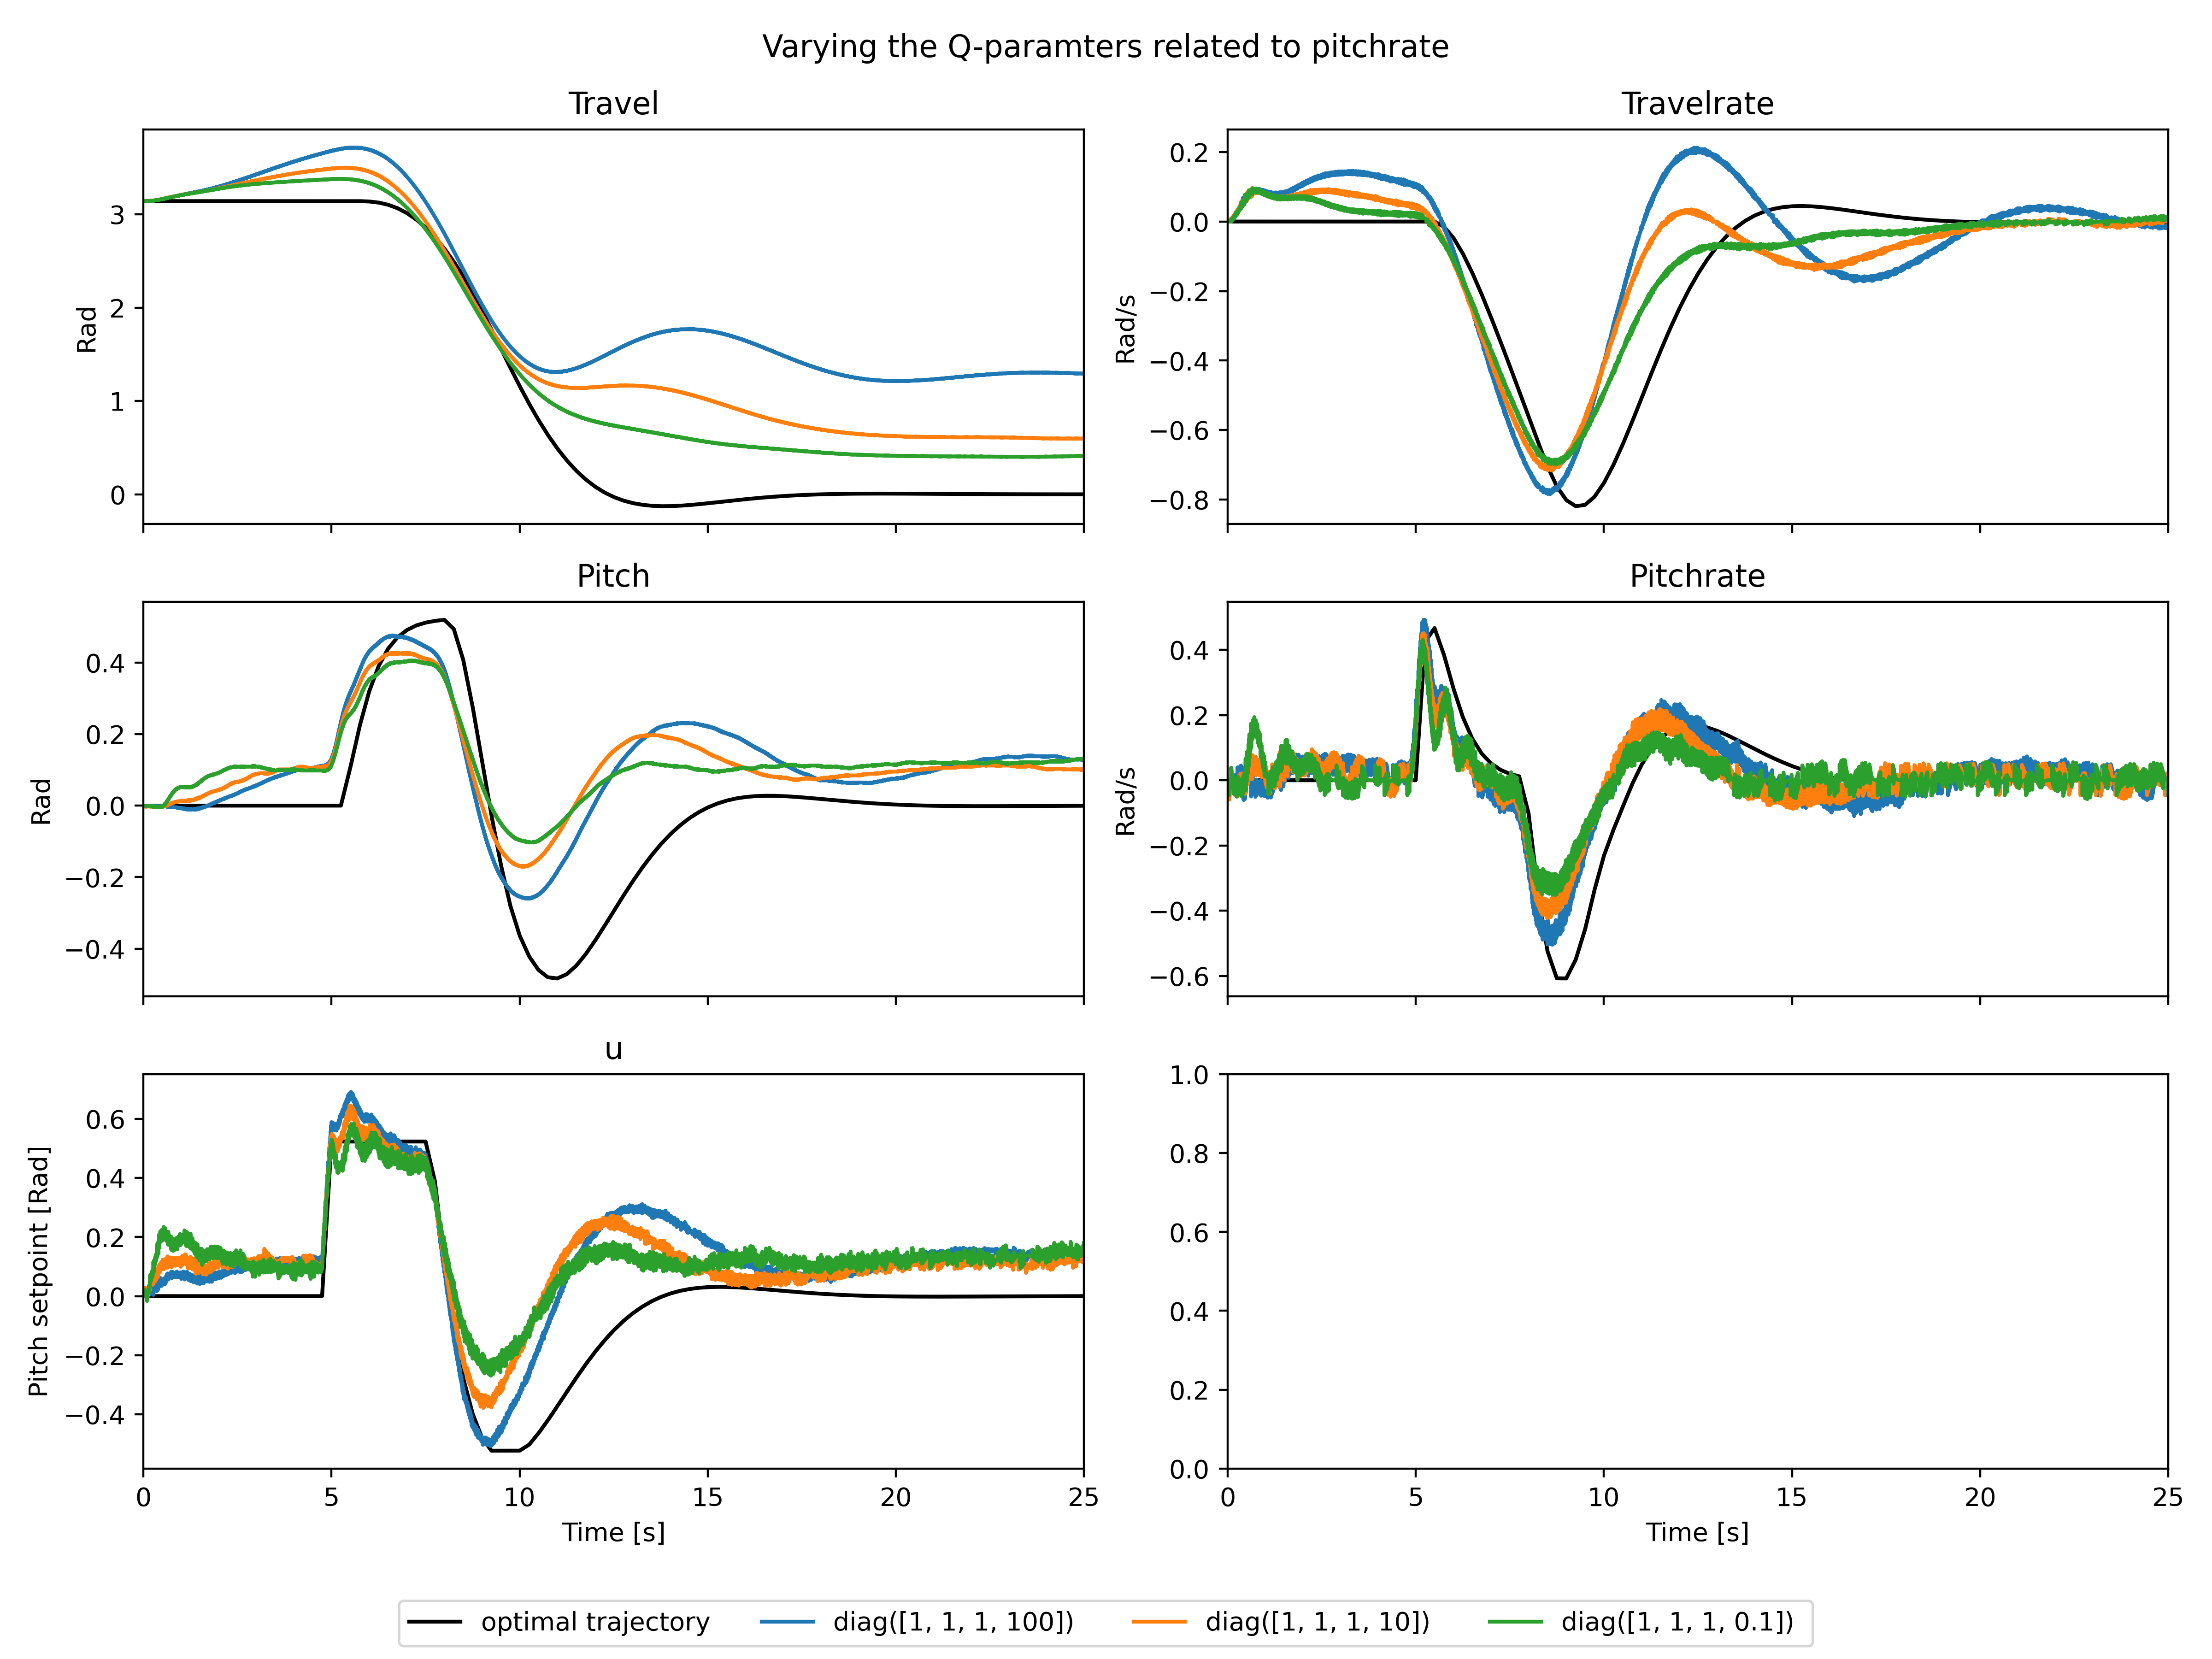
\includegraphics[width=0.8\linewidth]{figures/LAB3_Q_variations_pitchrate.png}
	\caption{Changing the weight of the pitchrate state, $R=1$. This was quite similar to \cref{fig:LAB3_Q_variations_pitch} but there is less oscillation.}
	\label{fig:LAB3_Q_variations_pitchrate}
\end{figure}
\subsubsection{Final tuning}
\todo[inline]{Oppgaven sier: ``.... Justify your choice''. Jeg tolker dette som at vi skal ha en final tuning.}
\missingfigure{Figure of final tuning}

\clearpage

\subsection{MATLAB and Simulink}
\lstinputlisting[caption= {MATLAB code for lab 3}, label={lst:lab3_matlab}]{code/problem_3.m}
\subsubsection{Simulink}
\begin{figure}[h]
	\centering
	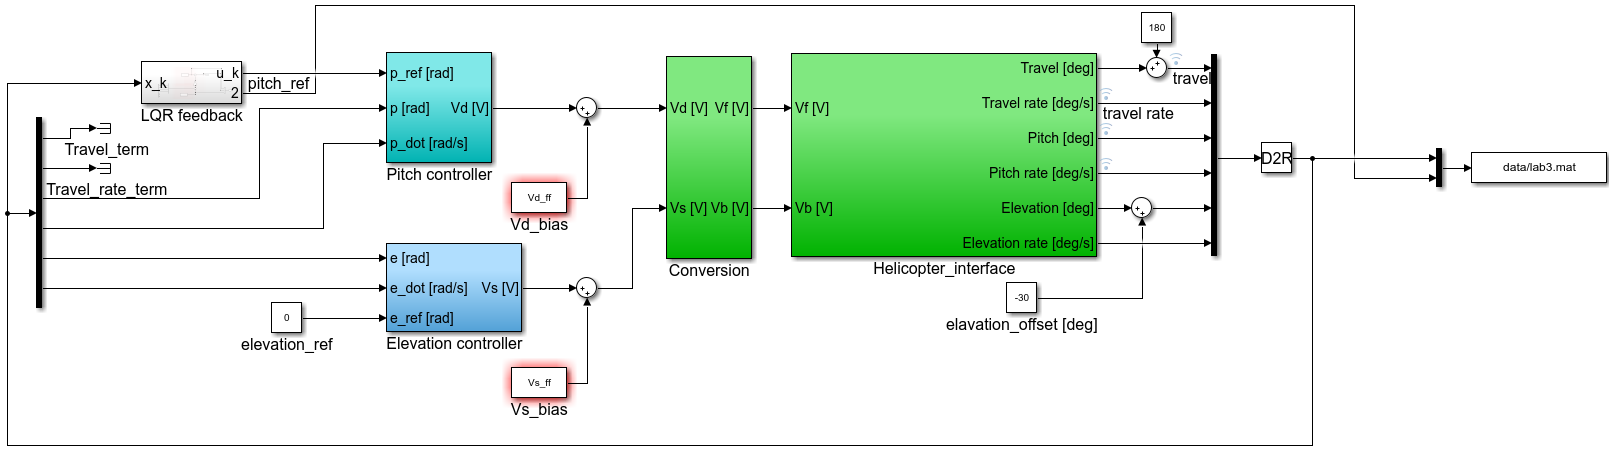
\includegraphics[width=1\linewidth, keepaspectratio]{code/lab3_simulink_1}
	\caption{Simulink diagram used in lab 3.}
	\label{fig:lab3_simulink}
\end{figure}
\begin{figure}[h]
	\centering
	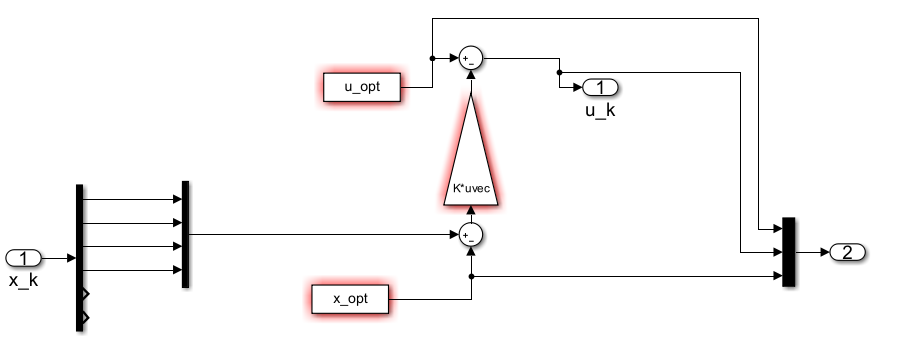
\includegraphics[width=1\linewidth, keepaspectratio]{code/lab3_simulink_2}
	\caption{``LQR Feedback'' subsystem in \cref{fig:lab3_simulink}}
	\label{fig:lab3_simulink_lqr}
\end{figure}
\end{document}